% 原书第54—62页：4.1.7—4.1.9。
\subsection{信息几何因果推断}

为了说明如何形式化 $P_{E\mid C}$ 与 $P_C$ 的独立性，本节介绍\textbf{信息几何因果推断（information-geometric causal inference，IGCI）}。IGCI，尤其是这里介绍的简单版本，是一种高度理想化的玩具场景；它清楚地展示了，一个方向上的独立性如何蕴含另一个方向上的相依性［Daniušis et al., 2010；Janzing et al., 2012］。它所依赖的假设确实很强：$X$ 和 $Y$ 在两个方向上都存在确定性关系，即
\[
 Y=f(X),\qquad X=f^{-1}(Y).
\]
也就是说，式 (3.2) 中的噪声变量是常量。此时，第4.1.2节所述的原因与机制独立性原理，就简化为 $P_X$ 与 $f$ 的独立性。值得注意的是，这种独立性会蕴含 $P_Y$ 与 $f^{-1}$ 的相依性。为了说明这一点，我们考察 Daniušis et al.［2010］所研究的一般场景中的下列特例。

\begin{definition}[信息几何因果推断模型]
如果满足以下条件，就称 $P_{X,Y}$ 满足从 $X$ 到 $Y$ 的 IGCI 模型。首先，$Y=f(X)$，其中 $f$ 是 $[0,1]$ 上的微分同胚，\footnote{如果一个函数可微、双射，而且其逆函数也可微，就称其为微分同胚。}
严格单调，且满足 $f(0)=0,f(1)=1$。此外，$P_X$ 具有严格为正的连续密度 $p_X$，并且满足以下“独立性条件”：
\begin{equation}
 \Cov[\log f',p_X]=0,
 \tag{4.10}
\end{equation}
其中，将 $\log f'$ 和 $p_X$ 看作赋予均匀分布的概率空间 $[0,1]$ 上的随机变量。\footnote{这种看法也许出乎意料，但请回忆，随机变量就是概率空间上的可测函数。这里，$\log f'$ 和 $p_X$ 都是 $x\in[0,1]$ 的函数，因此，它们都是同一概率空间 $[0,1]$ 上的随机变量。于是，$[0,1]$ 上的任何一个分布，都能为这些随机变量定义一个联合分布。}
\end{definition}

注意，式 (4.10) 中的协方差具体为
\[
\begin{aligned}
 \Cov[\log f',p_X]
 &=\int_0^1\log f'(x)p_X(x)\,\mathrm{d}x
   -\int_0^1\log f'(x)\,\mathrm{d}x
    \int_0^1p_X(x)\,\mathrm{d}x\\
 &=\int_0^1\log f'(x)p_X(x)\,\mathrm{d}x
   -\int_0^1\log f'(x)\,\mathrm{d}x.
\end{aligned}
\]
下面的结论由 Daniušis et al.［2010］和 Janzing et al.［2012］证明。

\begin{theorem}[信息几何因果推断模型的可识别性]
假设分布 $P_{X,Y}$ 容许从 $X$ 到 $Y$ 的 IGCI 模型。那么，逆函数 $f^{-1}$ 满足
\begin{equation}
 \Cov[\log (f^{-1})',p_Y]\geq0,
 \tag{4.11}
\end{equation}
且等号成立，当且仅当 $f$ 为恒等映射。
\end{theorem}

% 中文 TikZ 重排：坐标及曲线提取自原 PDF，未重新模拟数据。
\begin{figure}[htbp]
\centering
\definecolor{chfourfig4c0}{rgb}{0.13669,0.12195,0.12529}
\definecolor{chfourfig4c1}{rgb}{0.90323,0.90668,0.91019}
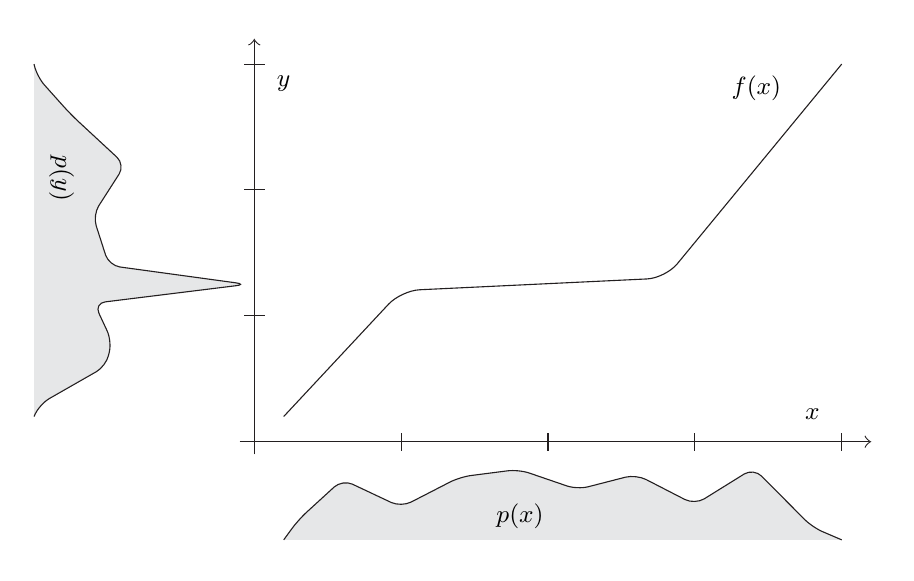
\begin{tikzpicture}[x=0.047cm,y=-0.047cm]
\useasboundingbox (0,0) rectangle (232,142);
\path[fill=none,draw=chfourfig4c0,line width=0.3985pt,draw opacity=1.0] (57.2782,111.8820) --(227.4671,111.8820);
\path[fill=none,draw=chfourfig4c0,line width=0.3188pt,draw opacity=1.0] (226.2716,110.2880) .. controls (226.3712,110.8857) and (227.4671,111.7824) ..(227.7660,111.8820) .. controls (227.4671,111.9816) and (226.3712,112.8783) ..(226.2716,113.4760);
\path[fill=none,draw=chfourfig4c0,line width=0.3985pt,draw opacity=1.0] (61.2470,115.2838) --(61.2470,3.4889);
\path[fill=none,draw=chfourfig4c0,line width=0.3188pt,draw opacity=1.0] (59.6530,4.6844) .. controls (60.2507,4.5848) and (61.1474,3.4889) ..(61.2470,3.1900) .. controls (61.3466,3.4889) and (62.2433,4.5848) ..(62.8410,4.6844);
\path[fill=none,draw=chfourfig4c0,line width=0.3985pt,draw opacity=1.0] (100.9324,114.2634) --(100.9324,109.5007);
\path[fill=none,draw=chfourfig4c0,line width=0.3985pt,draw opacity=1.0] (140.6177,114.2634) --(140.6177,109.5007);
\path[fill=none,draw=chfourfig4c0,line width=0.3985pt,draw opacity=1.0] (180.3031,114.2634) --(180.3031,109.5007);
\path[fill=none,draw=chfourfig4c0,line width=0.3985pt,draw opacity=1.0] (219.9884,114.2634) --(219.9884,109.5007);
\path[fill=none,draw=chfourfig4c0,line width=0.3985pt,draw opacity=1.0] (58.4688,77.8659) --(64.0253,77.8659);
\path[fill=none,draw=chfourfig4c0,line width=0.3985pt,draw opacity=1.0] (58.4688,43.8498) --(64.0253,43.8498);
\path[fill=none,draw=chfourfig4c0,line width=0.3985pt,draw opacity=1.0] (58.4688,9.8338) --(64.0253,9.8338);
\path[fill=none,draw=chfourfig4c0,line width=0.3985pt,draw opacity=1.0] (69.1839,105.0789) --(97.5277,74.7106) .. controls (99.4081,72.6960) and (103.1608,70.9568) ..(105.9098,70.8259) --(167.3887,67.8979) .. controls (170.1377,67.7671) and (173.7863,65.9365) ..(175.5382,63.8091) --(219.9884,9.8338);
\path[fill=chfourfig4c1,fill opacity=1.0,draw=chfourfig4c0,line width=0.3985pt,draw opacity=1.0] (69.1839,138.4145) --(71.3840,135.3973) .. controls (72.3608,134.0577) and (74.1424,132.0669) ..(75.3633,130.9507) --(82.8479,124.1080) .. controls (84.0687,122.9918) and (86.2695,122.6579) ..(87.7634,123.3622) --(98.2274,128.2952) .. controls (99.7213,128.9996) and (102.1244,128.9574) ..(103.5949,128.2011) --(114.1437,122.7758) .. controls (115.6142,122.0195) and (118.1348,121.2356) ..(119.7738,121.0249) --(129.7132,119.7471) .. controls (131.3522,119.5364) and (133.9477,119.8000) ..(135.5105,120.3358) --(145.7249,123.8380) .. controls (147.2878,124.3739) and (149.8528,124.4744) ..(151.4543,124.0626) --(161.5296,121.4716) .. controls (163.1310,121.0598) and (165.6212,121.3391) ..(167.0917,122.0954) --(177.6405,127.5206) .. controls (179.1110,128.2769) and (181.4403,128.1833) ..(182.8433,127.3114) --(193.6368,120.6042) .. controls (195.0397,119.7324) and (197.1213,119.9765) ..(198.2862,121.1496) --(209.9423,132.8887) .. controls (211.1072,134.0617) and (213.2852,135.5414) ..(214.8071,136.1937) --(219.9884,138.4145);
\path[fill=chfourfig4c1,fill opacity=1.0,draw=chfourfig4c0,line width=0.3985pt,draw opacity=1.0] (1.7190,105.0789) --(2.0393,104.3924) .. controls (2.7390,102.8928) and (4.4687,101.0128) ..(5.9028,100.1934) --(18.5684,92.9559) .. controls (20.0025,92.1364) and (21.4692,90.1681) ..(21.8445,88.5594) --(22.0728,87.5818) .. controls (22.4480,85.9731) and (22.1849,83.4534) ..(21.4852,81.9537) --(19.2572,77.1794) .. controls (18.5574,75.6798) and (19.3187,74.2999) ..(20.9577,74.0973) --(56.2951,69.7287) .. controls (57.9341,69.5261) and (57.9357,69.1804) ..(56.2988,68.9566) --(24.9222,64.6650) .. controls (23.2853,64.4412) and (21.5494,62.9852) ..(21.0450,61.4131) --(18.5061,53.4996) .. controls (18.0018,51.9274) and (18.3161,49.5259) ..(19.2082,48.1356) --(24.7084,39.5641) .. controls (25.6005,38.1738) and (25.3390,36.1341) ..(24.1241,35.0082) --(13.8399,25.4785) .. controls (12.6251,24.3526) and (10.7462,22.4404) ..(9.6432,21.2074) --(4.5100,15.4682) .. controls (3.4070,14.2351) and (2.2086,11.9315) ..(1.8332,10.3228) --(1.7190,9.8337);
\node[font=\small,inner sep=0pt,rotate=0] (ch04f4t0) at (69.1837,15.0379) {$y$};
\node[font=\small,inner sep=0pt,rotate=0] (ch04f4t1) at (212.0347,104.4399) {$x$};
\node[font=\small,inner sep=0pt,rotate=0] (ch04f4t2) at (196.9277,16.3515) {$f(x)$};
\node[font=\small,inner sep=0pt,rotate=0] (ch04f4t3) at (133.0587,132.0056) {$p(x)$};
\node[font=\small,inner sep=0pt,rotate=-90] (ch04f4t4) at (9.1484,40.8267) {$p(y)$};
\end{tikzpicture}
\caption{IGCI 思想的示意图：如果 $p_X$ 的选择独立于 $f$，那么，$p_Y$ 的峰往往出现在 $f$ 斜率较小、$f^{-1}$ 斜率较大的区域。因此，$p_Y$ 含有有关 $f^{-1}$ 的信息。IGCI 可以推广到 $f$ 不可微的情形［Janzing et al., 2015］。}
\label{fig:ch04-4}
\end{figure}


换言之，$\log f'$ 与 $p_X$ 不相关，会蕴含 $\log(f^{-1})'$ 与 $p_Y$ 正相关，只有平凡情形 $f=\mathrm{id}$ 例外。图4.4展示了这一点。还可以证明［Janzing and Schölkopf, 2015］，$f'$ 与 $p_X$ 不相关，即式 (4.10) 去掉对数后的对应条件，会蕴含 $(f^{-1})'$ 与 $p_Y$ 正相关；不过，IGCI 使用对数导数，是因为这样可以得到多种信息论解释［Janzing et al., 2012］。

为了论证式 (4.10) 的合理性，Janzing et al.［2012］描述了一个模型，其中随机生成 $f$ 的过程与 $P_X$ 独立，并证明在这种情况下，式 (4.10) 以较高概率近似成立。不过，应当强调，这类论证所涉及的模型总是过度简化的，未必能够描述现实情况。注意，IGCI 很容易推广到向量值变量之间的双射关系，Daniušis et al.［2010，第3节］已经给出了这种推广；但在经验数据中，双射的确定性关系很少见。因此，IGCI 只是一个玩具场景，用来说明：借助近似的独立性假设，可以实现原因—结果推断。IGCI 的假设还被用于解释［Janzing and Schölkopf, 2015］，为什么半监督学习的性能依赖于因果方向，见第5.1节。

我们绝不是要说，式 (4.10) 就是原因与机制独立性的正确形式化；我们也不认为，这种形式化只有唯一一种。例如，Sgouritsa et al.［2015］提出了一种“无监督逆回归”技术：尝试根据 $P_X$ 预测 $P_{Y\mid X}$，以及根据 $P_Y$ 预测 $P_{X\mid Y}$；随后，将预测性能较差的方向推断为因果方向。因此，这种方法把“独立性”解释为无法进行这类无监督预测。

\subsection{迹方法}

对于原因 $C$ 和结果 $E$ 都是高维变量、并通过线性结构因果模型相联系的情形，Janzing et al.［2010］和 Zscheischler et al.［2011］描述了 $P_C$ 与 $P_{E\mid C}$ 之间一种与 IGCI 有关的独立性。

\begin{definition}[迹条件]
设变量 $X$ 和 $Y$ 分别取值于 $\RR^d$ 和 $\RR^e$，满足线性模型
\begin{equation}
 Y=AX+N_X,\qquad N_X\indep X,
 \tag{4.12}
\end{equation}
其中，$A$ 是由结构系数组成的 $e\times d$ 矩阵。如果协方差矩阵 $\Sigma_{XX}$ 与 $A$ 在以下意义下“独立”，
\begin{equation}
 \tau_e(A\Sigma_{XX}A^{\mathsf T})
 =\tau_d(\Sigma_{XX})\tau_e(AA^{\mathsf T}),
 \tag{4.13}
\end{equation}
就称 $P_{X,Y}$ 满足从 $X$ 到 $Y$ 的\textbf{迹条件（trace condition）}。这里，$\tau_k(B):=\tr(B)/k$ 表示矩阵 $B$ 的归一化迹。
\end{definition}

一个违反迹条件的简单例子，是矩阵 $A$ 沿 $\Sigma_{XX}$ 的大特征值所对应的全部特征向量方向收缩，却沿小特征值所对应的特征向量方向拉伸。这当然意味着，$A$ 的选择并不独立于 $\Sigma_{XX}$。粗略地说，式 (4.13) 描述的是：$\Sigma_{XX}$ 的特征值，与 $A$ 改变相应特征向量长度的倍数，二者之间不相关。更形式化地，可以通过一个生成模型论证式 (4.13)：当 $d,e$ 很大时，按照适当的、旋转不变的先验概率，独立地随机选取 $\Sigma_{XX}$ 和 $A$。此时，它们以较高概率近似满足式 (4.13)［Besserve et al.，准备中］。

对于确定性的可逆关系，因果方向具有可识别性。

\begin{theorem}[通过迹条件获得的可识别性]
设 $X,Y$ 都是 $d$ 维变量，且 $Y=AX$，其中 $A$ 可逆。如果从 $X$ 到 $Y$ 的迹条件 (4.13) 成立，那么，反向模型
\[
 X=A^{-1}Y
\]
满足
\[
 \tau_d(A^{-1}\Sigma_{YY}A^{-\mathsf T})
 \leq\tau_d(\Sigma_{YY})\tau_d(A^{-1}A^{-\mathsf T}),
\]
且等号成立，当且仅当 $A$ 的所有奇异值具有相同的绝对值。
\end{theorem}
\begin{proof}
将 Janzing et al.［2010］的定理2应用于 $n:=m:=d$ 的情形，并注意到：只要 $Z$ 是严格为正、且并非几乎必然为常量的随机变量，$\Cov[Z,1/Z]$ 就为负，即可得证。
\end{proof}

因此，在一般情形下，反方向会违反迹条件，而且偏离等式的方向始终相同。

对于有噪声的关系，目前尚无类似定理4.12的结论。我们仍然可以检查式 (4.13) 是否在某个方向上近似成立，并把该方向推断为因果方向。此时，从 $Y$ 到 $X$ 的因果模型的结构矩阵不再是 $A^{-1}$。在这种情况下，记从 $X$ 到 $Y$ 的模型矩阵为 $A_X$，从 $Y$ 到 $X$ 的模型矩阵为 $A_Y$。确定性情形尤其方便，因为我们知道，下面的比值
\[
 \frac{\tau(A_X\Sigma_{YY}A_X^{\mathsf T})}
 {\tau(A_XA_X^{\mathsf T})\tau(\Sigma_{YY})}
\]
小于1，这是由于 $A_X=A_Y^{-1}$。\chfourtnote{原书上一句对 $A_X,A_Y$ 的方向定义，与本式及第4.2.3节不一致。本式中 $A_X$ 实际对应从 $Y$ 到 $X$ 的矩阵，而 $A_Y$ 对应从 $X$ 到 $Y$ 的矩阵；这也与第4.2.3节使用的下标约定一致。}
% 本段矩阵方向与原书后文4.2.3不一致，保留并在报告中标明。

本书提到的式 (4.10)、(4.13) 等独立性条件，其理论依据都依赖于高度理想化的生成模型。例如，式 (4.13) 的一种论证采用了这样一个模型：原因的协方差矩阵由旋转不变的先验分布生成［Janzing et al., 2010］。不过，我们仍然可以期待，理想化假设被违反，并不必然使因果推断方法失效。

Beuchet 椅子的比喻或许有助于说明这一点。首先，考虑在球面上均匀选择观察位置的情形。显然，这一选择不包含有关物体朝向的信息。在这个意义上，均匀先验形式化了一种“独立性”假设。此时，椅子的错觉只会出现在占比可以忽略的少量视角中。不难看出，要得到这一结论，并不要求观察位置的选择严格均匀。只要随机选择所依据的先验不集中在这少数特殊视角上，就会得到同样的结果。换句话说，关于一个典型观察者会看到什么的结论，对于底层独立性假设的违背具有稳健性。因此，讨论因果推断中的理想化假设时，应当关注的是，违反假设在多大程度上会使推断方法失效，而不是仅仅解释这些假设为什么过于理想化。

\subsection{算法信息论作为一种可能的基础}

本节介绍一个独立性原理。它以明确的数学形式为基础，但目前尚不清楚如何在实际中应用。因此，它介于两类讨论之间：一类是第2.1节关于因果推断基础的非形式化哲学讨论，另一类是第4.1.3—4.1.8节依赖相当具体的模型假设、关于原因与结果可能存在的不对称性的具体结论。

对于比第4.1.7和4.1.8节更一般的模型，要形式化“$P_E$ 与 $P_{C\mid E}$ 互不包含有关对方的信息”，并非易事。\chfourtnote{原书此处写的是 $P_E$ 与 $P_{C\mid E}$，但本节随后提出的因果机制独立性原理针对的是 $P_C$ 与 $P_{E\mid C}$。两组方向在原文中并不一致。}为此，需要一个适用于随机变量之外其他对象的信息概念。这是因为，$P_E$ 与 $P_{C\mid E}$ 本身不是随机变量，而是描述随机变量分布的对象。Kolmogorov 复杂度提供了一种有意思的信息概念，下面作简要介绍。
% 此处 P_E、P_{C|E} 为原书印刷符号；后文原理改用 P_C、P_{E|C}。

\paragraph{算法信息论中的概念}
先介绍\textbf{Kolmogorov 复杂度（Kolmogorov complexity）}。考虑一台通用 Turing 机 $T$，它是计算机的一种抽象，并且在拥有无限存储空间这个意义上是理想化的。对于任意二进制串 $s$，将 $K_T(s)$ 定义为一个最短程序的长度；\footnote{程序以二进制串给出，采用前缀无关编码，即任何一个程序的编码都不是另一个程序编码的前缀。否则，就需要额外的符号标记编码的结束位置。}
把这样的程序记为 $s^*$，使 $T$ 运行它后输出 $s$ 并停机［Solomonoff, 1964；Kolmogorov, 1965；Chaitin, 1966；Li and Vitányi, 1997］。可以把 $s^*$ 称为 $s$ 的最短压缩，但应记住，$s^*$ 包含了 $T$ 执行解压缩所需要的全部信息。因此，
\[
 K_T(s):=|s^*|,
\]
其中，$|\cdot|$ 表示二进制串的位数。这就针对给定的 Turing 机 $T$，定义了一个不依赖概率的信息量概念。以下固定一台 $T$，因此省略下标。虽然 $K(s)$ 不可计算，即不存在根据 $s$ 计算 $K(s)$ 的算法［Li and Vitányi, 1997］，但它仍然可以像本节这样，用于形式化一些概念性想法。

给定 $t$ 时 $s$ 的\textbf{条件算法信息（conditional algorithmic information）}记为 $K(s\mid t)$，定义为：以字符串 $t$ 为输入，生成输出 $s$ 后停机的最短程序的长度。进而可定义互信息为\footnote{注意，以 $t^*$ 为条件而非以 $t$ 为条件，二者存在区别，因为不存在根据 $t$ 计算 $t^*$ 的算法，反过来却可以。因此，作为输入，$t^*$ 可能比 $t$ 更有价值。事实表明，$K(s\mid t^*)$ 与条件 Shannon 熵之间的类比，比 $K(s\mid t)$ 更为密切。}
\[
 I(s:t):=K(s)-K(s\mid t^*).
\]
特别地，有［Chaitin, 1966］：
\begin{equation}
 I(s:t)\chfouraeq K(s)+K(t)-K(s,t),
 \tag{4.14}
\end{equation}
其中，符号 $\chfouraeq$ 表示等式仅在相差一个常数的意义下成立。也就是说，存在一个误差项，其大小的上界不依赖于 $s$ 和 $t$ 的长度。为定义字符串对 $(s,t)$ 的 Kolmogorov 复杂度 $K(s,t)$，可以先对字符串进行某种枚举，再利用 $\mathbb{N}$ 与 $\mathbb{N}\times\mathbb{N}$ 之间的标准双射，构造字符串与字符串对之间的简单双射。

式 (4.14) 的一个简单解释是：算法互信息衡量，把 $s,t$ 联合压缩，相比将它们各自独立压缩，能够节省多少存储空间。Janzing and Schölkopf［2010］认为，如果两个对象的二进制描述 $s,t$ 具有显著的互信息，那么这两个对象很可能存在因果联系。换言之，正如随机变量之间的统计相依关系表明它们之间存在因果联系，见原理1.1，对象之间的算法相依关系也表明这些对象之间存在因果联系。例如，若看到由不同公司生产的两件 T 恤具有相似图案，就可能意味着其中一家公司模仿了另一家公司。事实上，只要事先约定了将图案编码为二进制串的“适当”方式，以及一台“适当”的 Turing 机，就可以用算法互信息描述现实生活中图案的相似性。至于“适当”究竟意味着什么这一难题，也可参见 Janzing et al.［2016］引言中对“相对因果性”的简要讨论。

\paragraph{条件分布的算法独立性}
Janzing and Schölkopf［2010］以及 Lemeire and Janzing［2013］针对多元因果结构提出了条件分布算法独立性原理。不过，即使在二元情形下，这一原理也有非平凡的推论。

设两个变量 $C,E$ 分别为原因和结果，并假定 $P_C$ 和 $P_{E\mid C}$ 可以分别由二进制串 $s,t$ 有限描述。在参数化场景中，$s,t$ 可以描述相应参数空间中的点。也可以把 $s,t$ 理解为程序，它们能对所有具有有限描述长度的取值 $c,e$，计算 $p(c)$ 与 $p(e\mid c)$。于是，用 $I(P_C:P_{E\mid C})$ 表示 $I(s:t)$，并提出以下原理。

\begin{principle}[算法独立的条件分布]
$P_C$ 与 $P_{E\mid C}$ 在算法意义下独立，即
\begin{equation}
 I(P_C:P_{E\mid C})\chfouraeq0,
 \tag{4.15}
\end{equation}
等价地，
\begin{equation}
 K(P_{C,E})\chfouraeq K(P_C)+K(P_{E\mid C}).
 \tag{4.16}
\end{equation}
\end{principle}

式 (4.15) 与式 (4.16) 的等价性是直接的，因为描述分布对 $(P_C,P_{E\mid C})$，等价于描述联合分布 $P_{C,E}$。原理4.13的思想是，$P_C$ 与 $P_{E\mid C}$ 是自然界中在因果上互不相关的对象。这当然是一种理想化假设。不过，在“$X$ 导致 $Y$”或“$Y$ 导致 $X$”的场景中，它提示我们：只要 $P_X$ 与 $P_{Y\mid X}$ 之间的算法相依弱于 $P_{X\mid Y}$ 与 $P_Y$ 之间的算法相依，就推断 $X\to Y$。然而，把这一思想应用于经验数据时，除了算法互信息不可计算之外，还面临另一个问题：有限数据无法确定 $P_{X,Y}$。

尽管存在这些问题，原理4.13仍然有助于为实际因果推断方法提供依据。下面以加性噪声模型为例说明。Janzing and Steudel［2010］指出，结构因果模型 $Y:=f_Y(X)+N_Y$ 意味着，$y\mapsto\log p(y)$ 的二阶导数，由 $(x,y)\mapsto\log p(x\mid y)$ 的偏导数确定。因此，知道 $P_{X\mid Y}$，就可以在一定精度下简短地描述 $P_Y$。只要 $K(P_Y)$ 大于这少量信息，Janzing and Steudel［2010］便据此认为，应当拒绝 $Y\to X$，因为 $P_Y$ 与 $P_{X\mid Y}$ 在算法意义下相依。对于任意给定的数据集，我们无法保证 $K(P_Y)$ 足够大，以至于仅凭存在一个从 $Y$ 到 $X$ 的加性噪声模型，就能够拒绝 $Y\to X$。\chfourtnote{原书这句话将已有加性噪声模型的方向写成 $Y\to X$。结合前文正在用正向模型排除反向因果解释的论证，此处应理解为存在从 $X$ 到 $Y$ 的加性噪声模型。正文保留原书方向。}但是，当把基于加性噪声模型原理的推断应用于大量不同分布时，我们知道，其中大多数 $P_Y$ 都足够复杂，因为低复杂度分布的集合很小。因此，可以据此拒绝那些在相反方向上诱导出加性噪声模型的因果模型。
% 上段“从Y到X”忠实保留原文，原书此处方向疑误见校对报告。
此外，图5.4左图和右图给出了两个简单的玩具例子：仅观察 $P_X$，就能够对联合分布 $P_{X,Y}$ 作出一种简单猜测。实际上，可以证明，这意味着 $P_X$ 与 $P_{Y\mid X}$ 之间存在算法相依；Janzing and Schölkopf［2010，式 (27) 后的注释］针对左图的情形给出了这一证明。

还应指出，式 (4.15) 蕴含
\begin{equation}
 K(P_C)+K(P_{E\mid C})
 \chfouraeq K(P_{C,E})
 \chfouraleq K(P_E)+K(P_{C\mid E}).
 \tag{4.17}
\end{equation}
等式成立，是因为描述 $P_{C,E}$ 等价于描述分布对 $(P_C,P_{E\mid C})$，其长度不会短于分别描述边缘分布与条件分布的长度。不等式成立，是因为 $P_E$ 与 $P_{C\mid E}$ 也能确定 $P_{C,E}$。换句话说，条件分布的独立性意味着，联合分布在因果方向上具有比反因果方向更短的描述。\footnote{检验式 (4.17) 左端是否小于右端，并非检验独立性的唯一方式。只要两个字符串在算法意义下独立，分别对它们应用复杂度为 $O(1)$ 的函数后，所得的两个字符串仍然在算法意义下独立，尽管可能变得更简单［Janzing and Schölkopf, 2010，引理6］。因此，原则上不必先知道字符串的复杂度，也能够拒绝算法独立性。}

从\textbf{最小描述长度原理（minimum description length principle）}［Grünwald, 2007］以及 Occam 剃刀的思想来看，这一推论也很自然。不过，条件 $K(P_C)+K(P_{E\mid C})\chfouraleq K(P_E)+K(P_{C\mid E})$ 严格弱于式 (4.15)。这是因为，$P_{C,E}$ 的最短描述可能并不采用这两种可能分解中的任何一种；例如，存在潜在共同原因时，就可能出现这种情况［Janzing and Schölkopf, 2010，第16页］。

原理6.53将原理4.13推广到了多元情形。
